\documentclass[a4j]{jsarticle}
\usepackage{graphicx}
\usepackage{listings}

\title{2024年度プログラミング\textsc{iii} 演習課題}
\author{学籍番号: 35714121 \\ 氏名: 福富隆大}
\date{2024年10月31日}

\begin{document}
\maketitle

\textbf{1 はじめに} \\

本レポートは演習課題第5回の実行結果をまとめたものである。\\

\textbf{2 課題の実行結果} \\

\textmd{(課題5-1)} \\

課題の実行結果を図1に示す。 \\

\begin{figure}[htbp]
  \centering
  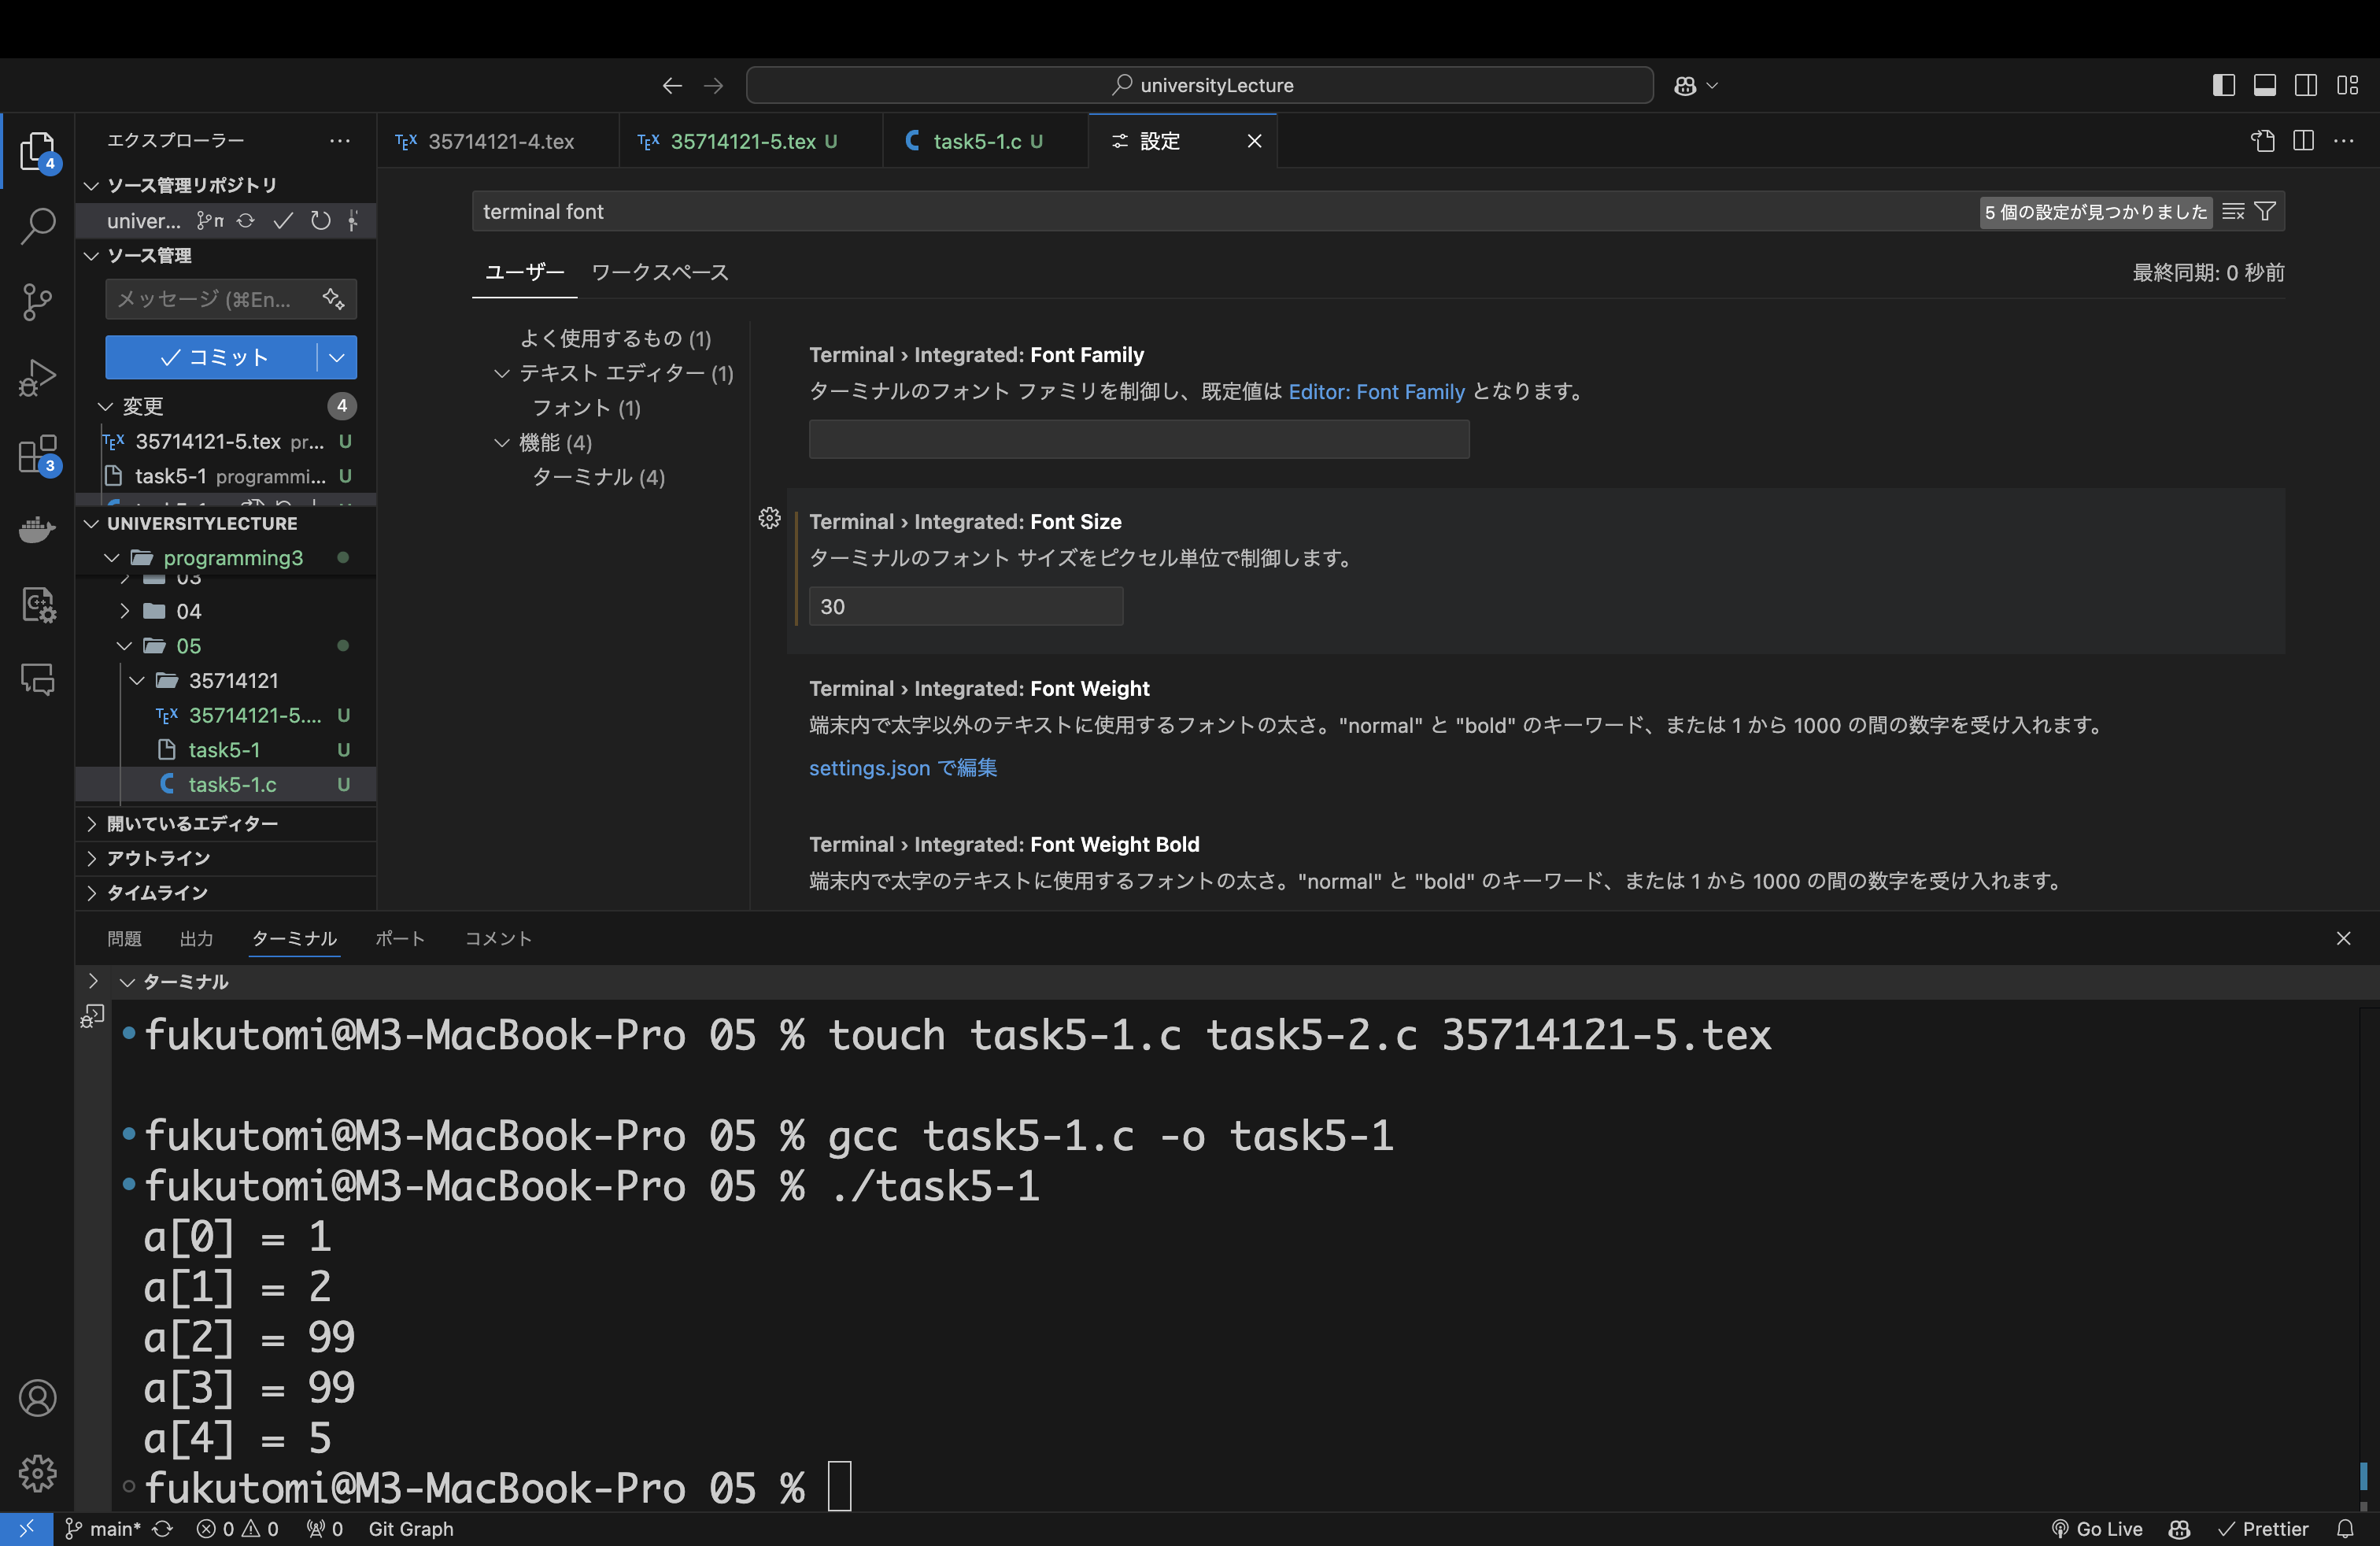
\includegraphics[width=10cm]{task5-1.eps}
  \caption{(ターミナルの部分に実行結果があります)}
  \label{fig:sample}
\end{figure}

\textmd{コードと結果の説明} \\
ary\_set(\&a[2], 2, 99)として配列のポインタを引数に指定したので、ary\_set関数内でV[0]=a[2]となりa[2]とa[3]の値が99になった。\\

\textmd{(課題5-2)} \\

課題の実行結果を図2に示す。\\

\begin{figure}[htbp]
  \centering
  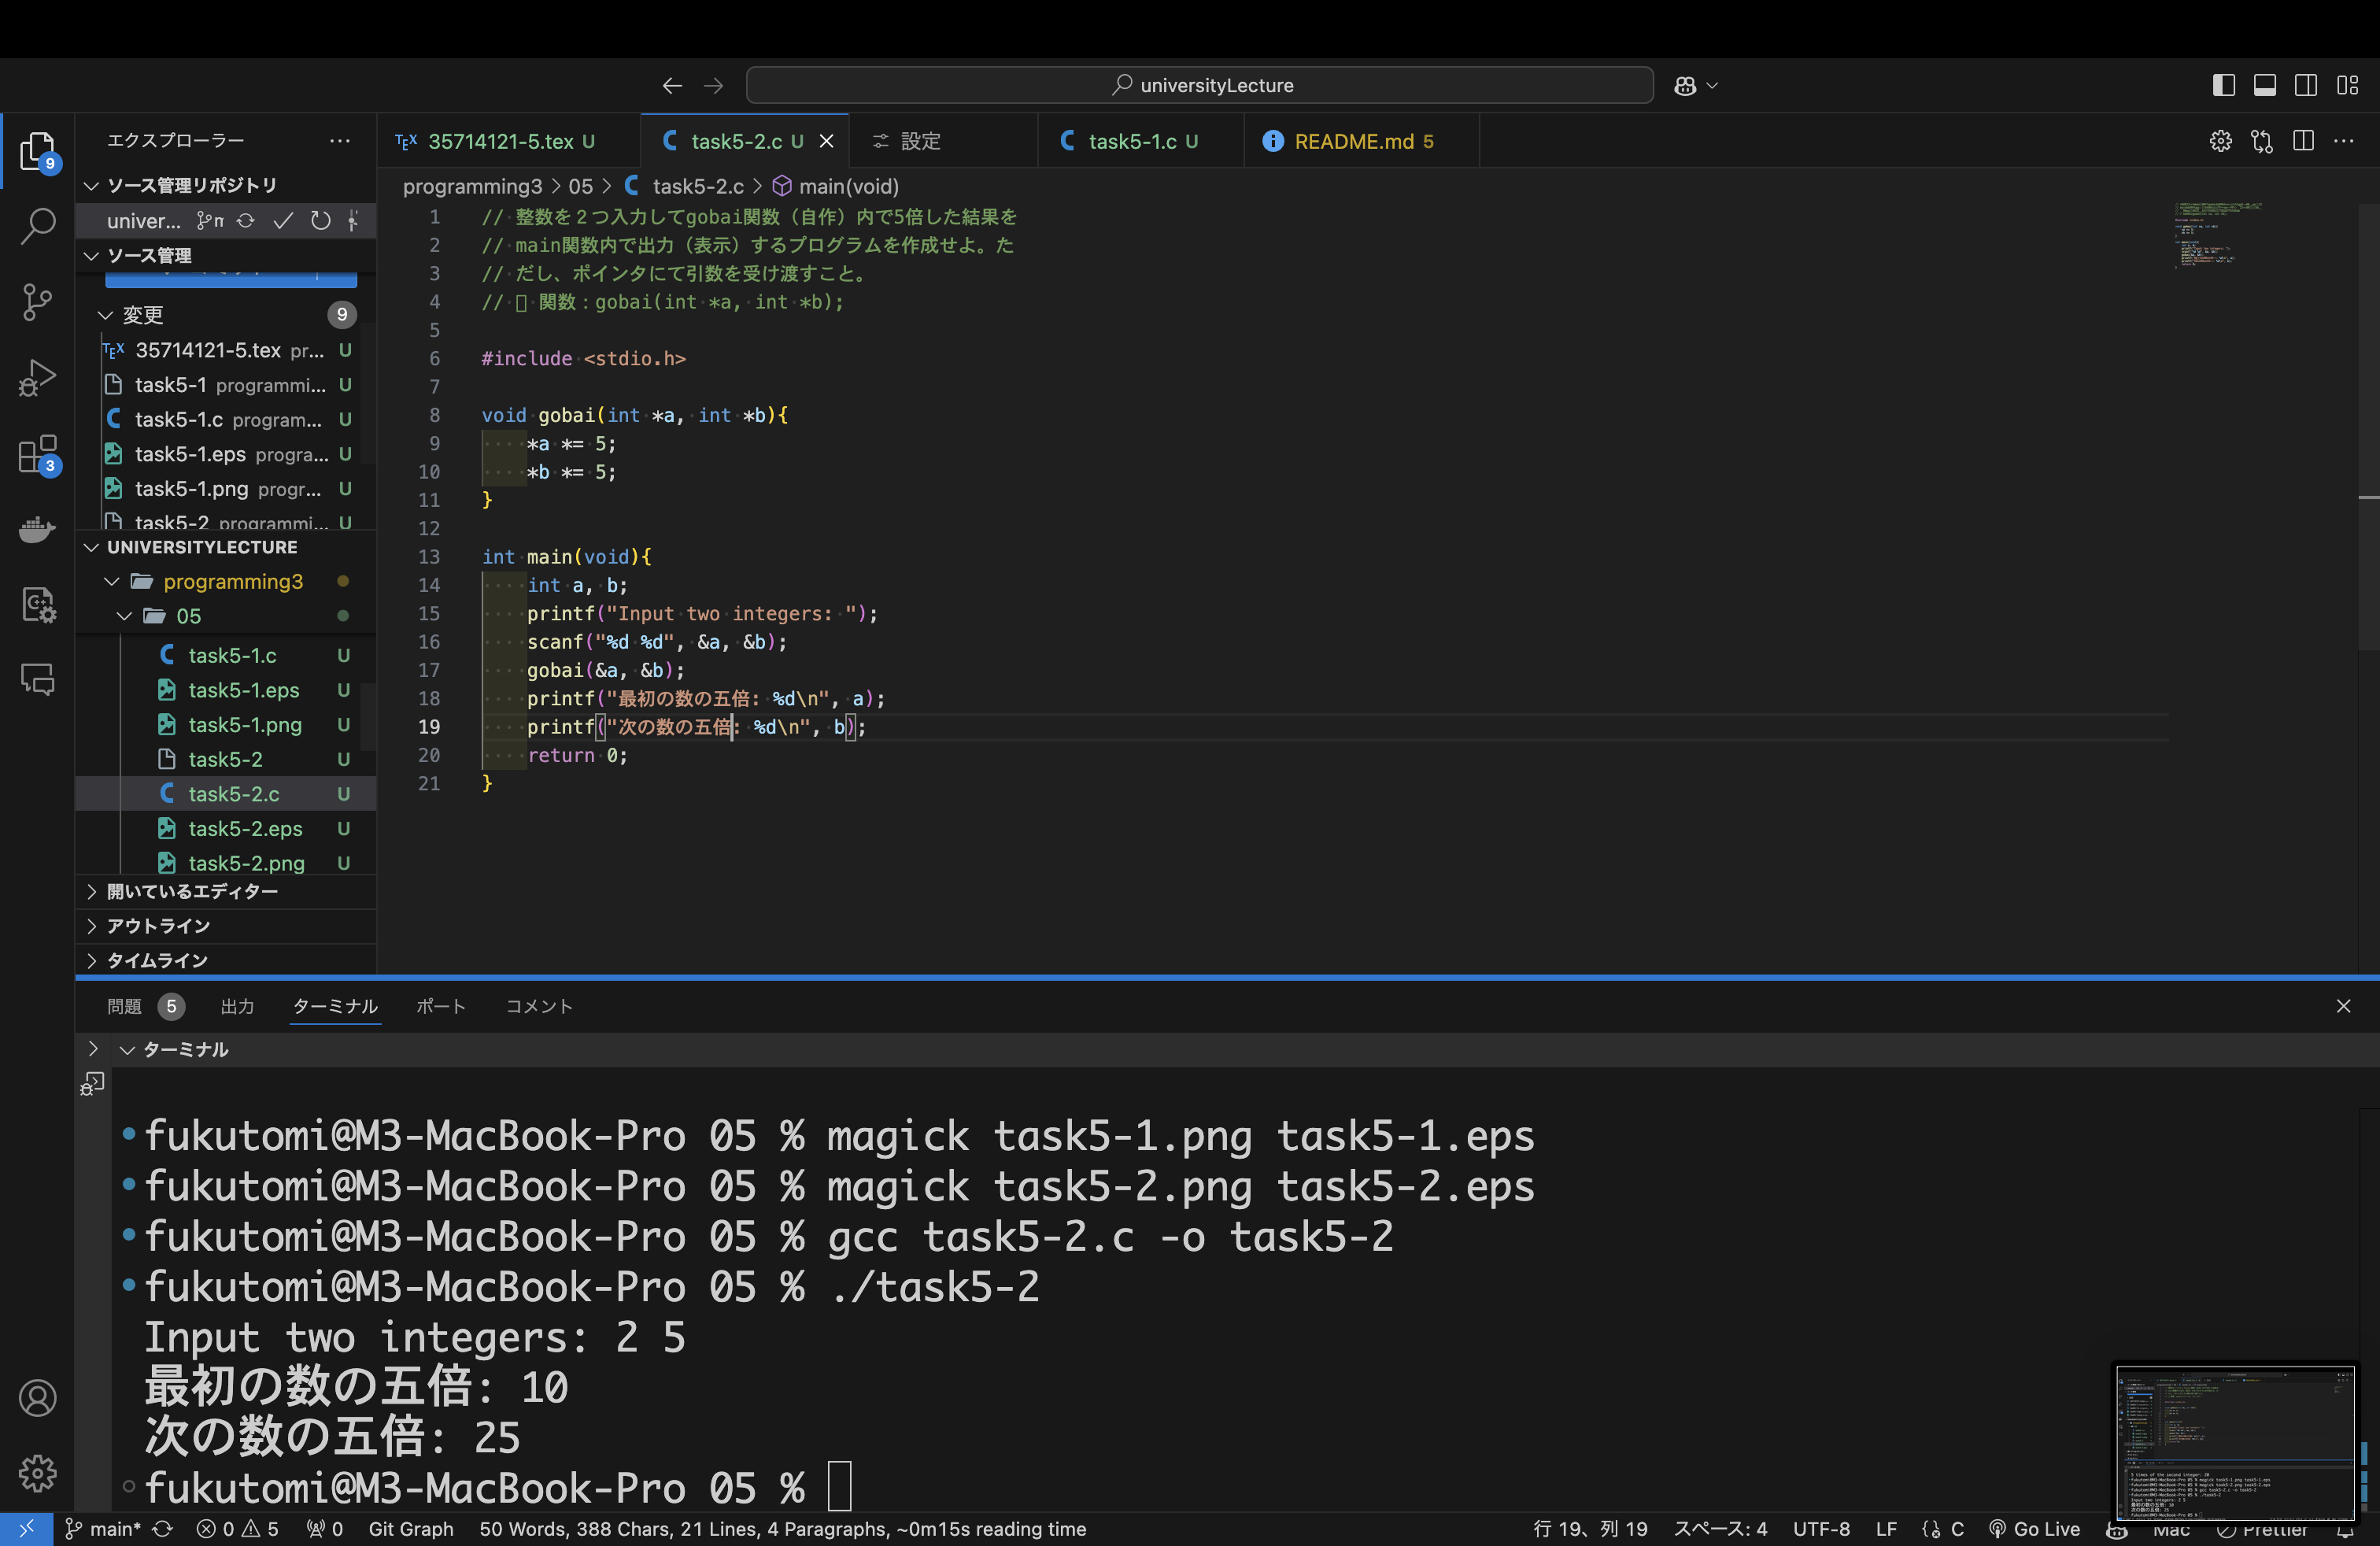
\includegraphics[width=10cm]{task5-2.eps}
  \caption{(ターミナルの部分に実行結果があります)}
  \label{fig:sample}
\end{figure}

\textmd{コードと結果の説明} \\
gobai関数は引数にポインタを指定し、関数内でポインタの中身を五倍している。\\
scanfで入力した値を読み込み、gobai関数に入力された値が格納してある変数のポインタを渡して実行した。\\
ポインタを引数に渡してもちゃんと五倍された値が出力されている。\\

\end{document}
